% !TEX program = lualatex
\documentclass[A4,svgnames,9pt,aspectratio=169]{beamer}

\usepackage[utf8]{inputenc}
\usepackage{amsmath,amssymb,amsfonts}
\usepackage{mathtools}
\usepackage{bm}
\usepackage{graphicx}
\usepackage{caption}
\usepackage{booktabs}
\usepackage{colortbl}
\usepackage{tikz}
\usetikzlibrary{positioning, shapes, arrows.meta, calc}

\hypersetup{
   allcolors=rouge_inria,
   pdfauthor   = {Louis Hauseux},
   pdftitle    = {De l'intérêt des bibliothèques de geometry processing puissantes pour un clustering hiérarchique fin : CGAL, Geogram, etc.},
   pdfsubject  = {Présentation à Bruno Lévy},
   pdfkeywords = {Louis Hauseux, clustering, Delaunay, percolation, optimal transport}
}

\title[Geometry Processing \& Clustering]{\large De l'intérêt des bibliothèques de \emph{geometry processing} puissantes\\[2pt] pour un clustering hiérarchique fin : CGAL, Geogram, \emph{etc.}\\[6pt] \normalsize \normalfont Ce qui leur manque encore pour passer aux interactions d'ordre supérieur.}
\subtitle{\small Présentation à \href{https://brunolevy.github.io/}{Bruno \textsc{Lévy}}\\[2pt]\footnotesize (Univ. Paris-Saclay, Inria Saclay, CNRS, LMO, Équipe \textsc{ParMa})}
\date[juin 2026]{Juin 2026}
\author[L. Hauseux]{%
   \small Louis \textsc{Hauseux} (Inria Sophia Antipolis, bourse 3IA--DS4H d'Université Côte d'Azur) \\[3pt]
   \footnotesize Encadré par \href{https://www-sop.inria.fr/members/Konstantin.Avratchenkov/me.html}{Konstantin \textsc{Avrachenkov}} (\textsc{Neo}) \& \href{https://www-sop.inria.fr/members/Josiane.Zerubia/index-eng.html}{Josiane \textsc{Zerubia}} (\textsc{Ayana})
}
\institute{Saclay}

\usetheme{inria}

\newcounter{tocsectioncounter}
\renewcommand{\contentsname}{Plan}
\setbeamertemplate{section in toc}{%
    \vspace*{2ex}%
    \setcounter{tocsectioncounter}{\inserttocsectionnumber}%
    \textcolor{inria-noir}{\textbf{\Roman{tocsectioncounter})~\inserttocsection}}%
}

\begin{document}

% Page de titre
\frame{\titlepage}

% Plan
\begin{frame}{Plan}
  \tableofcontents
\end{frame}

\section{Clustering : des statistiques aux graphes}
\frame{\sectionpage}

\begin{frame}{Clustering sur données euclidiennes $X \subset \mathbb{R}^d$}
    \begin{columns}
        \begin{column}{0.50\textwidth}
            \begin{block}{Modèle de Hartigan \cite{hartigan81}}
                \begin{itemize}
                    \item Estimation de la densité $f$ par $K$-NN.
                    \item Définition des \textbf{amas de forte densité} (\emph{high-density clusters}) comme composantes connexes des ensembles de niveau de $f$ \cite{HDBSCAN, HDBSCAN2017}.
                    \item Seuil de percolation et graphes géométriques aléatoires \cite{penrose2003}.
                \end{itemize}
            \end{block}
            
            \vspace{0.1cm}
            \begin{center}
                \begin{tikzpicture}[node distance=0.1cm, every node/.style={inner sep=0}]
                    \node (raw) {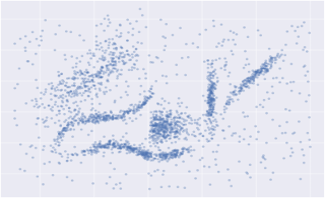
\includegraphics[width=0.43\linewidth]{../Img_presentation_BrunoLevy/Nuage2D.png}};
                    \node [right=of raw] (arrow) {\small $\xrightarrow{\text{HDBSCAN}}$};
                    \node [right=of arrow] (clustered) {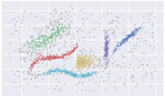
\includegraphics[width=0.43\linewidth]{../Img_presentation_BrunoLevy/Nuage2D_HDBSCAN.png}};
                \end{tikzpicture}
            \end{center}
        \end{column}
        
        \begin{column}{0.46\textwidth}
            \begin{exampleblock}{Exemples d'applications}
                \begin{itemize}
                    \item \textbf{Données réelles} : classification des huiles d'olive italiennes ($\mathbb{R}^8$) \cite{tourr}, où la géographie forme la vérité terrain.
                    \item \textbf{Cosmologie} : extraction des filaments galactiques en 3D.
                \end{itemize}
            \end{exampleblock}
            
            \vspace{0.1cm}
            \begin{center}
                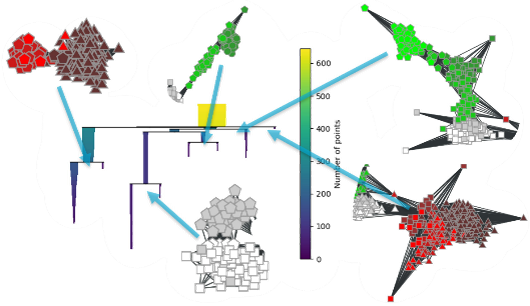
\includegraphics[width=0.47\linewidth]{../Img_presentation_BrunoLevy/CondenseTree_OliveOil_HGP.png}
                \hfill
                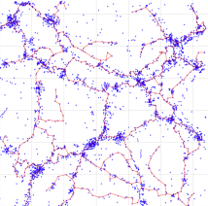
\includegraphics[width=0.47\linewidth]{../Img_presentation_BrunoLevy/FilamentsGalaxie.png}
            \end{center}
        \end{column}
    \end{columns}
\end{frame}

\section{HDBSCAN \& quelques applications en 3D}
\frame{\sectionpage}

\section{Vers des interactions d'ordre supérieur}
\frame{\sectionpage}

\section{La mosaïque de \textnormal{\textsc{Delaunay}} d'ordre supérieur}
\frame{\sectionpage}

\begin{frame}[allowframebreaks]{Références}
    \bibliographystyle{apalike}
    \bibliography{referencesThesis}
\end{frame}

\end{document}
